\chapter{Navrhování algoritmů}
\label{chap:navrhovanialgoritmu}
	V této kapitole se budeme zabývat problematikou návrhu algoritmů ve výpočetní geometrii. Abychom byli schopni jednotlivé algoritmi mezi sebou porovnávat co se týče rychlosti a nároků na paměť, bude zde zmíněna asymptotická složitost. Dále zde budou představeny nejznámější techniky návrhů algoritmů ve výpočetní geometrii, které nám mohou usnadnit práci a dostat na problém jiný pohled.

\section{Časová a prostorová složitost algoritmů}
	Abychom mohli porovnávat algoritmy, řešící stejný problém, mezi sebou a rozhodnout se kdy který algoritmus použít, slouží nám k tomuto účelu základní dvě míry pro porovnání.
\begin{itemize}
	\item časová složitost
	\item prostorová složitost
\end{itemize}
	Časová složitost vyjadřuje jak dlouho bude výpočet podle daného algoritmu trvat, obdobně prostorová složitost nám vyjadřuje kolik prostoru, tedy paměti, danému algoritmu budeme muset poskytnout pro výpočet. Je očividné že vyjadřovat časovou složitost v sekundách a prostorovou v bytech by vzhledem k různému hardwaru, či různé implementaci nebylo příliš vhodné. Pro popis složitosti algoritmu tedy používáme \textit{Asymptotickou složitost}.
	
\subsection{Asymptotická složitost}
	Asymptotická složitost se vyjadřuje jako matematická funkce, popisující závislost využití paměťového prostoru nebo výpočetního výkonu na velikosti vstupních dat $N$. Důležité je že tato funkce je neklesající a vyjadřujeme ji pouze jako třídu složitosti, tedy typ funkce a ne jako přesné vyjádření. Pro příklad funkce $f(x)=1000N^2$ nebo $g(x)=N^2 + 1000N$ jsou třídy složitosti $\mathcal{O} (N^2)$. Tedy zanedbáváme multiplikativní konstantu, aditivní konstantu a nižší řády funkce, protože nás zajíma jak se bude měnit časová složitost vzhledem ke zvětšujícím vstupním datům.
	
	Tím že zanedbáváme multiplikativní, aditivní konstantu a nižší řády funkce, může se vyskytnout případ kdy algoritmus s vyžším řádem asymptotické složitosti proběhne rychleji než algoritmus s nižším řádem. Máme ovšem jistotu že existuje vstup o velikosti $N_0$, kde toto přestane platit. Při praktickém použití tato situace může nastat v případě, kdy asymptoticky rychlejší algoritmus má složitější implementaci a prostředky vynaložené na režiji převyšují výhody algoritmu. Takováto situace je vyjádřena na obrázku \ref{fig:4-time_complexity}, kde vidíme že díky zanedbaným multiplikativním a aditivním konstantám může být reálný čas výpočtu asymptoticky rychlejšího algoritmu menší než algoritmu s vyžší asymptotickou časovou složitostí. Je zde ovšem vidět že při velikosti vstupu $N_0$ se situace obrátí a dále se chovají tak, jak bysme očekávali.\cite{hartmanis1965on}
	
\begin{figure}[h]
  \centering
  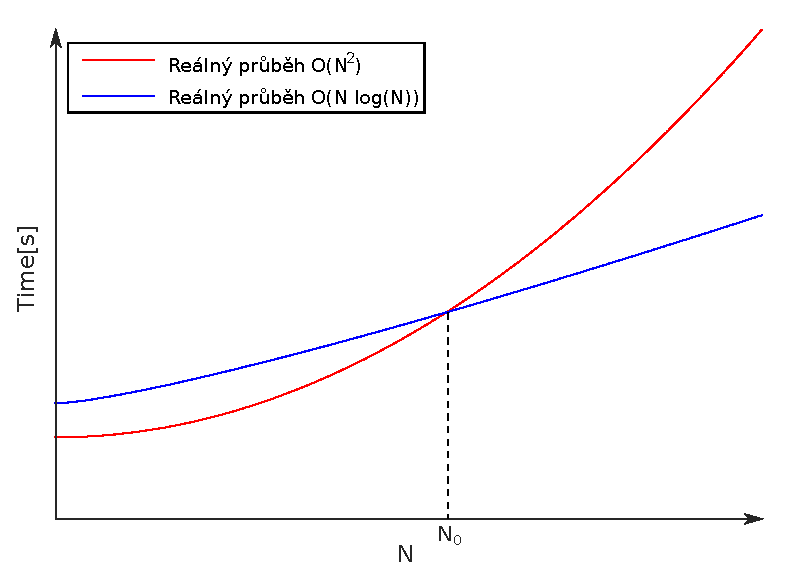
\includegraphics[width=10cm]{./pictures/4/time_complexity.pdf}
  \caption{Graf znázorňující časový průběh algoritmu v závislosti na velikosti vstupu $N$}
  \label{fig:4-time_complexity}
\end{figure}
	
	 Pro vyjádření časové složitosti můžeme využít různé varianty.
\begin{itemize}
	\item Horní odhad složitosti - $\mathcal{O} (f(N))$
	\item Průměrná složitost - $\Theta (f(N))$
	\item Dolní odhad složitosti - $\Omega (f(N))$
\end{itemize}	
	Často vídané vyjádření složitosti je takzvaná \textit{Omikron notace}, která vyjadřuje horní odhad, tedy nejhorší možný případ jakým se může algoritmus chovat. V tomto případě máme jistotu že algoritmus bude asymptoticky probíhat stejně rychle nebo rychleji v případě časové složitosti. V některých případech se vyplatí uvádět i průměrnou složitost, tedy složitost, která nastává při náhodném rozložení vstupních dat. Typickou ukázkou, kde je vhodné využít průměrnou časovou složitost je metoda \textit{Quick-Sort}, která patří mezi třídící algoritmy. Horní odhad složitosti je $\mathcal{O}(n^2)$. Při vhodné implementaci se ovšem lze kvadratické složitosti účinně bránit a obecně se algoritmus chová s průměrnou časovou složitostí $\Theta (n \log n)$ což je pro třídící algoritmy nejlepší možné.\cite{wirth1989algoritmy} Poslední variantou je dolní odhad složitosti, který nám naopak vyjadřuje že algoritmus se bude chovat stejně nebo hůře než je uvedeno. Toto vyjádření využijeme především v oblasti kryptografie.\cite{milkova2010algoritmy} \cite{bayer2008algoritmy}
	
\subsection{Stanovení časové složitosti}
	Pro určení časové složitosti je nutné určit počet operací v závislosti na velikosti vstupních dat. Nezajímame se o přesný počet operací, ale o vztahu počtu operací k velikosti vstupní množiny. Pro komplikované algoritmy to může být nesnadný úkol. U geometrických algoritmů se často zajímáme pouze o horní odhad složitosti, díky jeho relativně jednoduchému zjištění oproti průměrnému odhadu.
	
	
\begin{table}

\begin{tabular}{ |p{1.4cm}||p{1.6cm}|p{1.6cm}|p{1.6cm}|p{1.6cm}|p{1.6cm}|p{1.6cm}|  }
% \hline
% \multicolumn{7}{|c|}{Závislost času výpočtu na asymptotické složitosti} \\
\hline

$N$				&10			&20			&40			&60			&500		&1000\\
\hline
$\log n$		&2,3µs		&4,3µs		&5µs		&5,8µs		&9µs		&10µs\\			
$n$				&10µs		&20µs		&40µs		&60µs		&0,5s		&1ms\\
$n \log n$		&23µs		&86µs		&0,2ms		&0,35ms		&4,5ms		&10ms\\
$n^2$			&0,1ms		&0,4ms		&1,6ms		&3,6ms		&0,25s		&1s\\
$n^3$			&1ms		&8ms		&64ms		&0,2s		&125s		&17min\\
$n^4$			&10ms		&160ms		&2,56s		&13s		&17h		&11,6dní\\
$2^n$			&1ms		&1s			&12,7 dní	&36000 let	&			&\\
$n!$			&3,6s		&77000 let	&			&			&			&\\
\hline

\end{tabular}
\caption{Příklad závislosti výpočetního času na asymptotické složitosti algoritmu}
\label{tab:4-time_complexity}
\end{table}

\section{Metody návrhů algoritmů ve výpočetní geometrii}
	Abychom byli schopni porozumět různým algoritmům, nebo navrhnout nový algoritmus pro různé operace ve výpočetní geometrii, je dobré seznámit se s často využívanými metodami, používané v algoritmech výpočetní geometrie. Metody návrhů alogritmů neřeší konkrétní problém, ale pouze obecný postup jak se při hledání řešení chovat.

\subsection{Metoda hrubé síly}
	Patří k nejjednodušším metodám algoritmizace. Jak vyplývá z názvu, v této metodě budeme postupovat hrubou silou, tedy v praxi to znamená že algoritmus bude zkoušet všechny možné kombinace řešení. Mezi výhody patří jednoduchá implementace a snadné porozumění algoritmu, které se často shoduje s definicí výsledku. Tyto algoritmy lze využívat zpravidla pro malé vstupní množiny, nebo pro ověření správnosti výsledku. V praxi lze algoritmy využít i jako doplněk složitějších algoritmů, kde by režije, jako je volání funkcí nebo vytváření objektů, zabralo více času než na tuto malou množinu použít algoritmus hrubé síly. Velmi často je časová složitost těchto algoritmů $\mathcal{O}(2^n)$ či dokonce $\mathcal{O}(n!)$. V tabulce \ref{tab:4-time_complexity} pak můžeme vidět že časová složitost pro větší vstupy je neúnosná.
	
\subsection{Heuristické algoritmy}
	Heuristické algoritmy se velmi podobají metodě hrubé síly, pouze nezkoumají všechna možná řešení. Tato technika je velmi často používaná u optimalizačních úloh, kde neexistuje exaktní řešení. Zatím co u algoritmu řešící úlohu metodou hrubé síly bylo nalezení optimálního řešení zaručeno, heuristické algoritmy hledají pouze přípustné řešení. Tímto způsobem docílíme lepší časové náročnosti oproti algoritmům hrubé síly. Jednou ze známých metod heuristických algoritmů jsou takzvané hladové algoritmy. Ty se nalezením lekálně optimálních řešení snaží docílit lokálního optima. Příkladem hladového algoritmu může být nalezení nepravidelné trojúhelníkové sítě nad množinou bodů v rovině, kdy postupně přidáváme do řešení nejkratší hrany, pokud ovšem nekříží jinou hranu vyskytující se již v řešení.
	
\begin{figure}[h]
    \centering % <-- added
\begin{subfigure}{0.25\textwidth}
  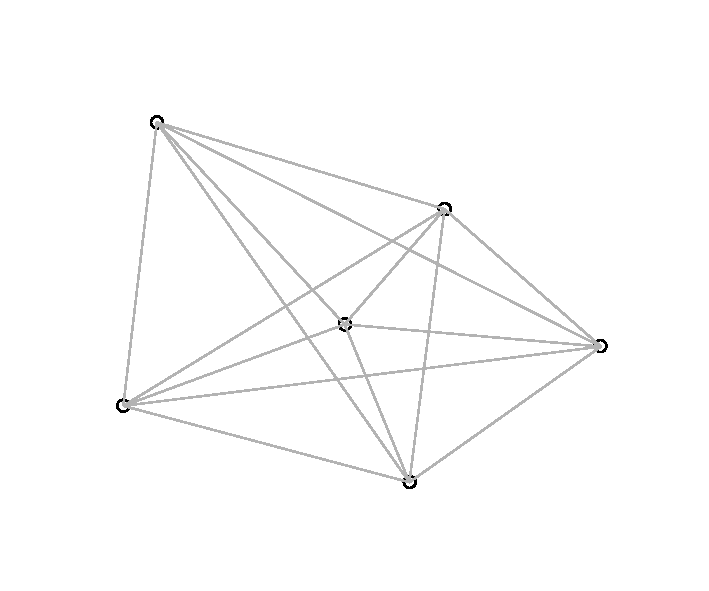
\includegraphics[width=\linewidth]{./pictures/4/triangulation_1.pdf}
  \label{fig:3-triangulation_1}
\end{subfigure}\hfil % <-- added
\begin{subfigure}{0.25\textwidth}
  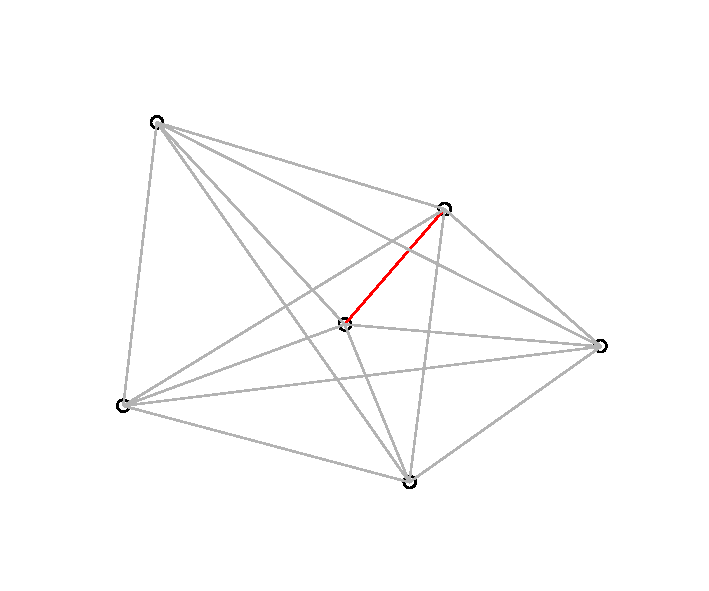
\includegraphics[width=\linewidth]{./pictures/4/triangulation_2.pdf}
  \label{fig:3-triangulation_2}
\end{subfigure}\hfil % <-- added
\begin{subfigure}{0.25\textwidth}
  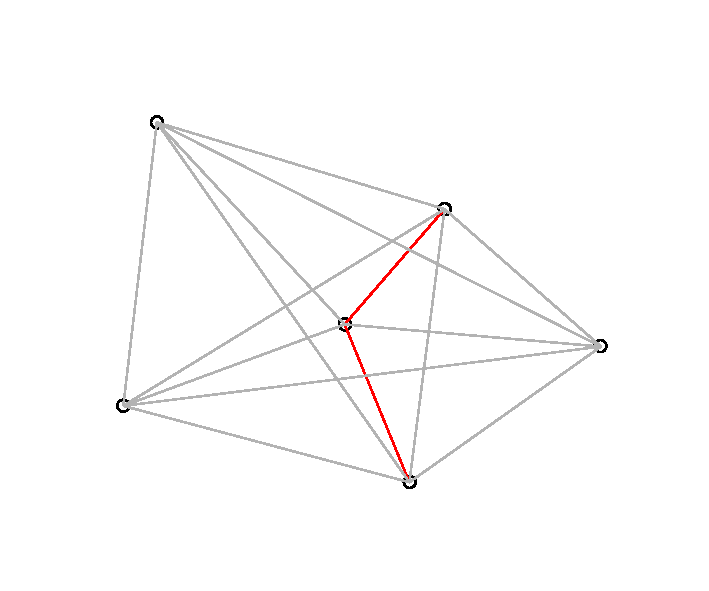
\includegraphics[width=\linewidth]{./pictures/4/triangulation_3.pdf}
  \label{fig:3-triangulation_3}
\end{subfigure}\hfil % <-- added
\begin{subfigure}{0.25\textwidth}
  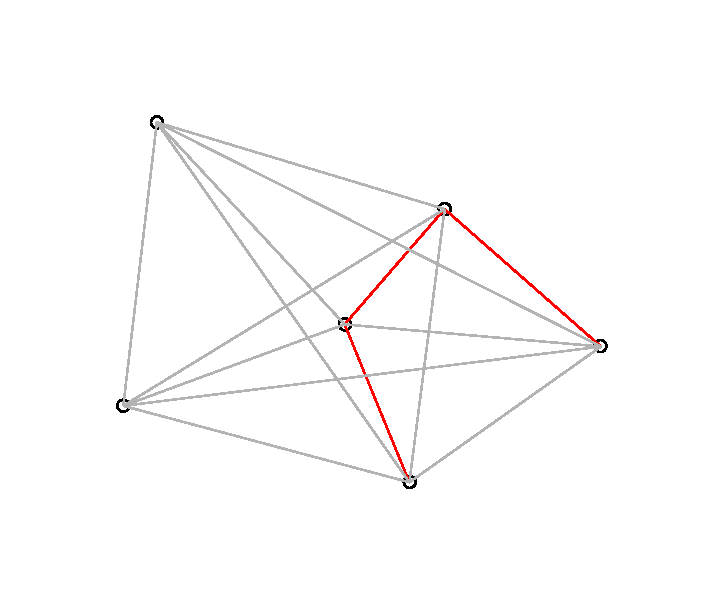
\includegraphics[width=\linewidth]{./pictures/4/triangulation_4.pdf}
  \label{fig:3-triangulation_4}
\end{subfigure}\hfil % <-- added
\begin{subfigure}{0.25\textwidth}
  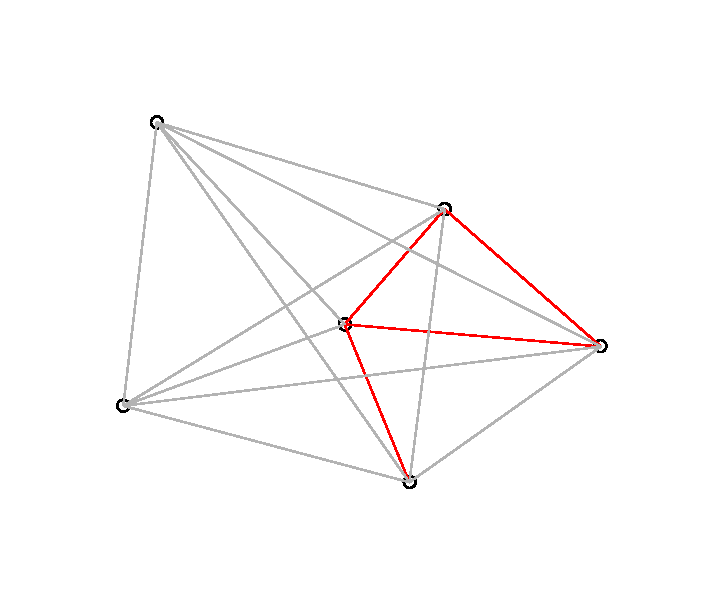
\includegraphics[width=\linewidth]{./pictures/4/triangulation_5.pdf}
  \label{fig:3-triangulation_5}
\end{subfigure}\hfil % <-- added
\begin{subfigure}{0.25\textwidth}
  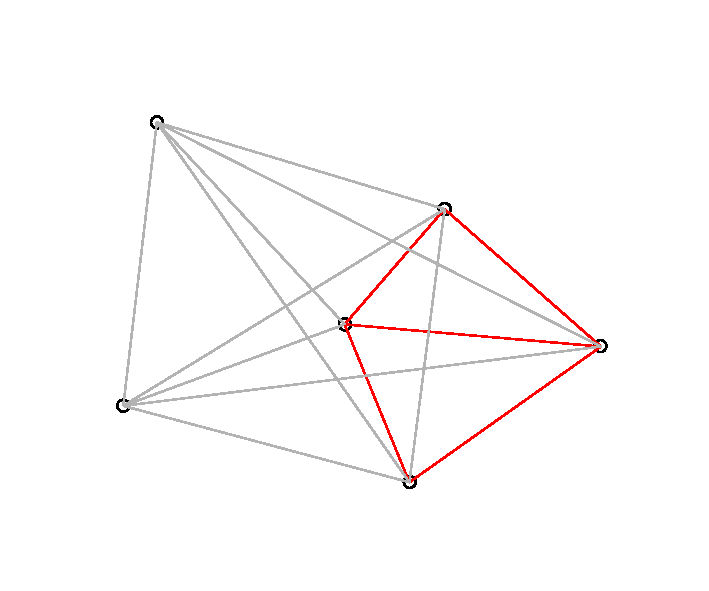
\includegraphics[width=\linewidth]{./pictures/4/triangulation_6.pdf}
  \label{fig:3-triangulation_6}
\end{subfigure}\hfil % <-- added
\begin{subfigure}{0.25\textwidth}
  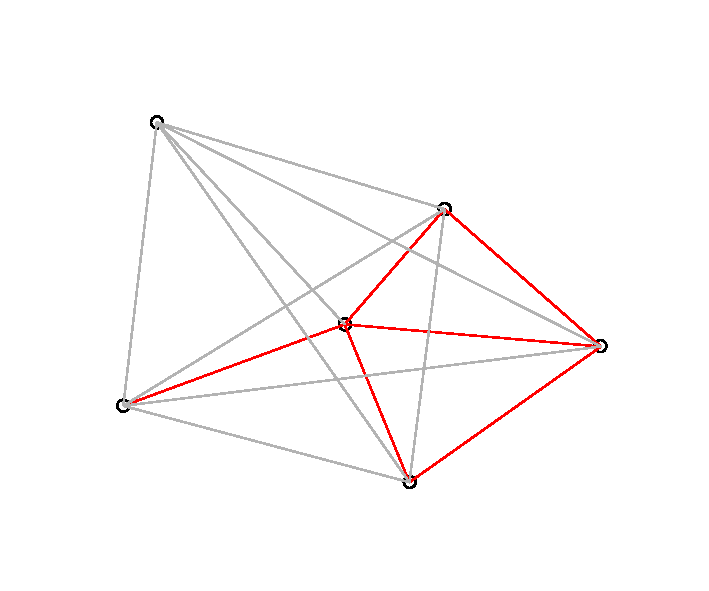
\includegraphics[width=\linewidth]{./pictures/4/triangulation_7.pdf}
  \label{fig:3-triangulation_7}
\end{subfigure}\hfil % <-- added
\begin{subfigure}{0.25\textwidth}
  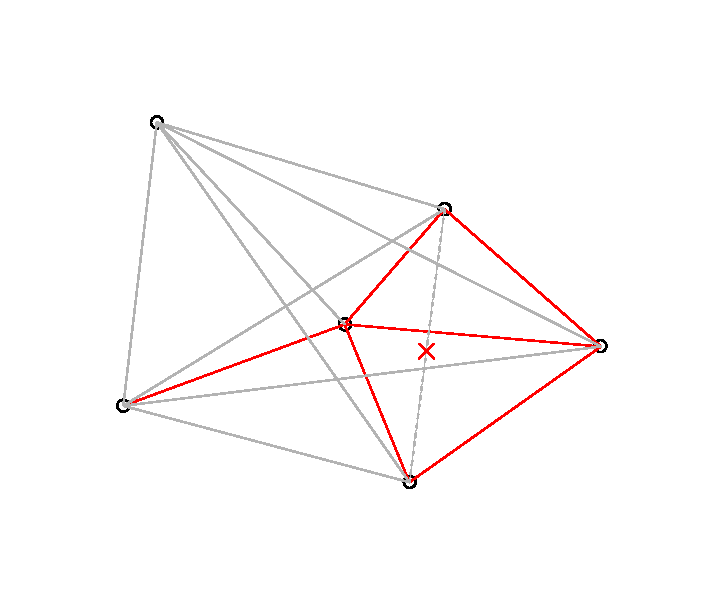
\includegraphics[width=\linewidth]{./pictures/4/triangulation_8.pdf}
  \label{fig:3-triangulation_8}
\end{subfigure}\hfil % <-- added
\begin{subfigure}{0.25\textwidth}
  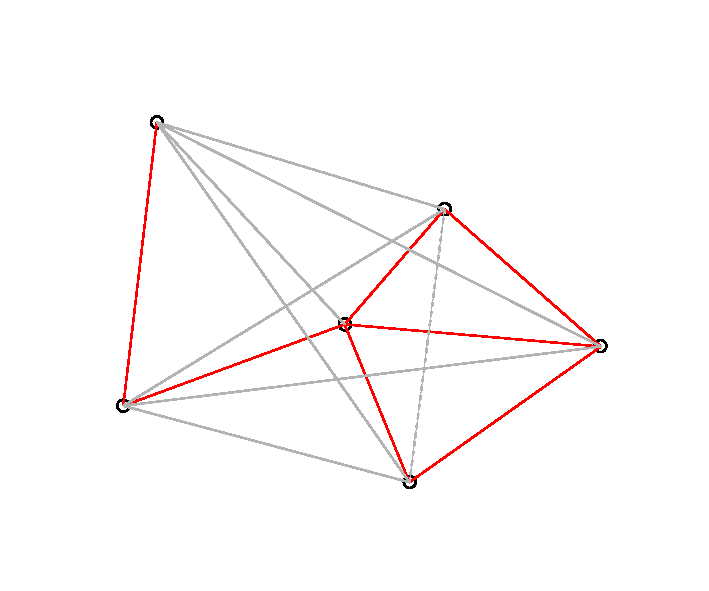
\includegraphics[width=\linewidth]{./pictures/4/triangulation_9.pdf}
  \label{fig:3-triangulation_9}
\end{subfigure}\hfil % <-- added
\begin{subfigure}{0.25\textwidth}
  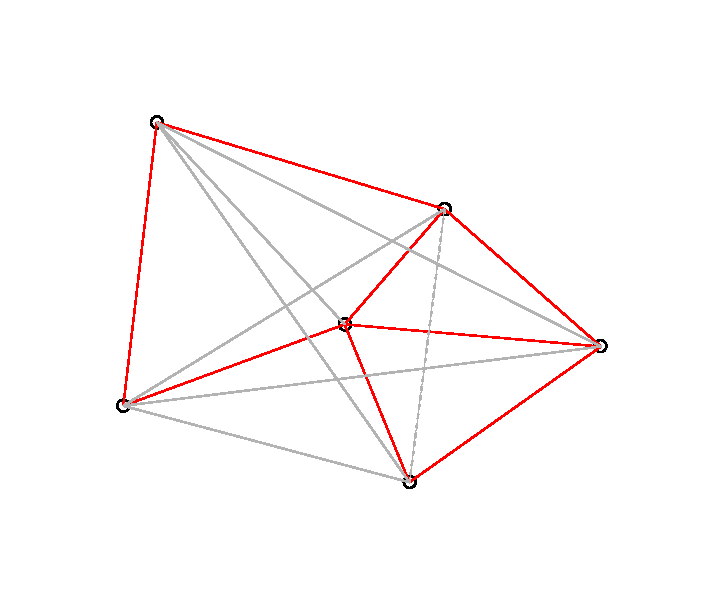
\includegraphics[width=\linewidth]{./pictures/4/triangulation_10.pdf}
  \label{fig:3-triangulation_10}
\end{subfigure}\hfil % <-- added
\begin{subfigure}{0.25\textwidth}
  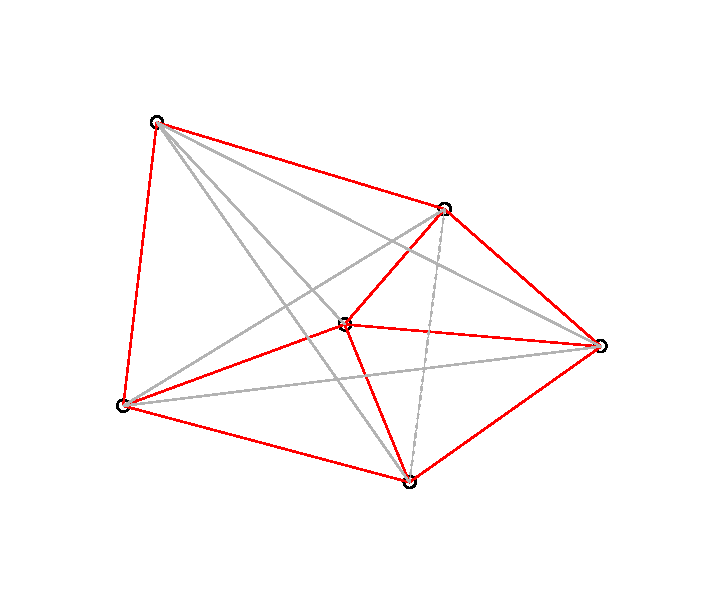
\includegraphics[width=\linewidth]{./pictures/4/triangulation_11.pdf}
  \label{fig:3-triangulation_11}
\end{subfigure}\hfil % <-- added
\begin{subfigure}{0.25\textwidth}
  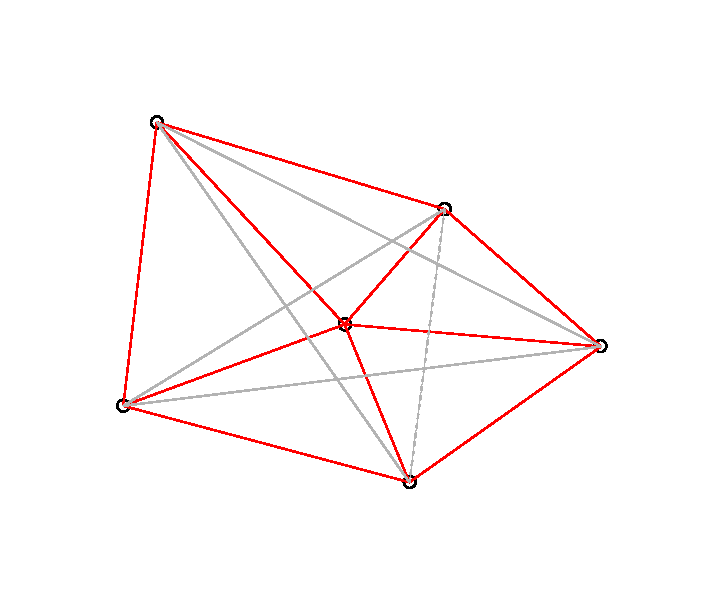
\includegraphics[width=\linewidth]{./pictures/4/triangulation_12.pdf}
  \label{fig:3-triangulation_12}
\end{subfigure}\hfil % <-- added

\caption{Znázornění postupu algoritmu pro nalezení triangulace metodou hladového algoritmu.}
\label{fig:3-triangulation}
\end{figure}	
	
	
	
\subsection{Rozděl a panuj}
	Nejen ve výpočetní geometrii je známá a hojně používaná metoda \textit{rozděl a panuj}, známá také pod anglickým názvem \textit{divide and conquer}. Paradigma je založeno na rekurzivním rozdělování problému na dvě či více částí, stejného nebo podobného typu, dokud nebudeme schopni problém jednoduše vyřešit. Řešení dílčích problémů se pak spojuje a získá se řešení původního problému. Metoda \textit{rozděl a panuj} je vhodná pro paralelní zpracování, kde pří každém rozdělení nám vznikají dvě či více částí, které můžeme řešit nezávisle na sobě.\cite{frigo1999cache}
	Do algoritmů této kategorie patří například generalizační algoritmus \textit{Douglas-Peucker}\cite{van1997algorithmic}, který je vhodný svou jednoduchostí na ukázkou metody rozděl a panuj. 
	Na vstupu dostává algoritmus linii, kterou chceme generalizovat a hodnotu vzdálenosti o kterou se generalizovaná linie může maximálně lišit od původní. Funkce vyhledá bod s maximální vzdáleností od úsečky spojující počáteční a koncový bod, který je zároveň vzdálenější než námi zadaná mez, poté se rekurzivně zavolá na dvě úsečky obsahující tento bod. Takto se postupuje do té doby dokud existuje bod s větší vzdáleností než zadaná mez. Po dokončení se řešení složí z jednotlivých kroků rekurze.

\begin{figure}[h]
    \centering % <-- added
\begin{subfigure}{0.5\textwidth}
  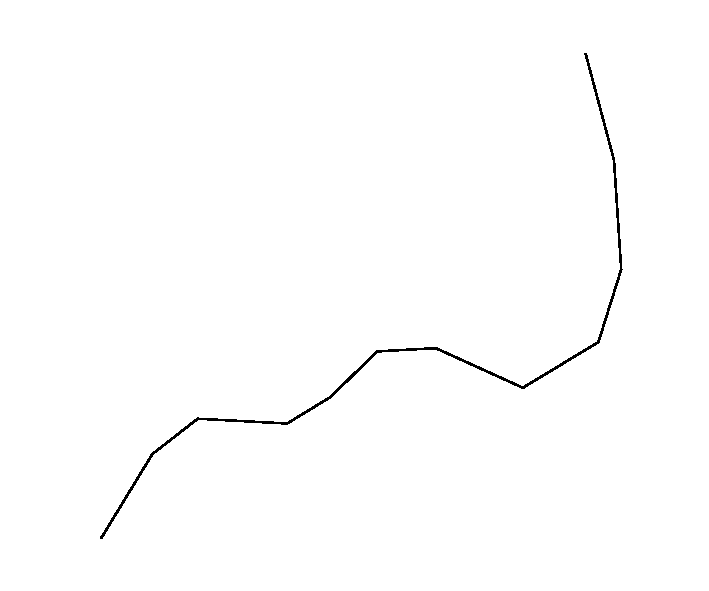
\includegraphics[width=\linewidth]{./pictures/4/douglas-peucker_1.pdf}
  \label{fig:3-douglas-peucker_1}
\end{subfigure}\hfil % <-- added
\begin{subfigure}{0.5\textwidth}
  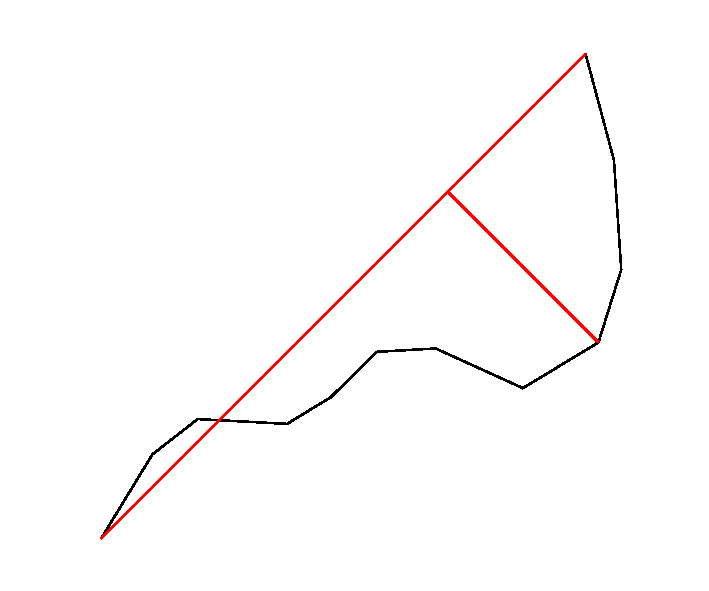
\includegraphics[width=\linewidth]{./pictures/4/douglas-peucker_2.pdf}
  \label{fig:3-douglas-peucker_2}
\end{subfigure}\hfil % <-- added
\begin{subfigure}{0.5\textwidth}
  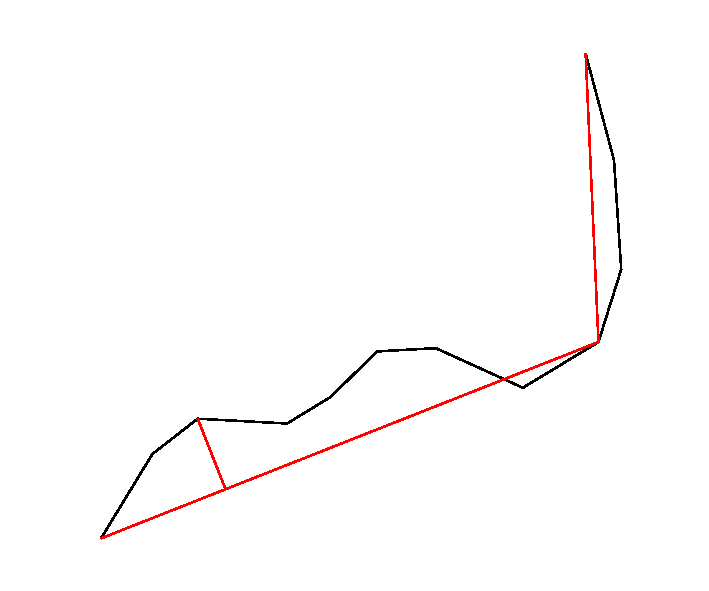
\includegraphics[width=\linewidth]{./pictures/4/douglas-peucker_3.pdf}
  \label{fig:3-douglas-peucker_3}
\end{subfigure}\hfil % <-- added
\begin{subfigure}{0.5\textwidth}
  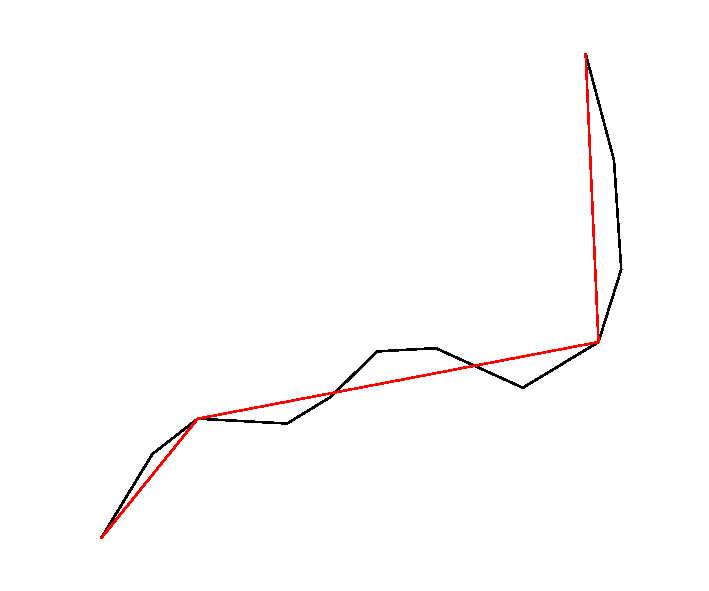
\includegraphics[width=\linewidth]{./pictures/4/douglas-peucker_4.pdf}
  \label{fig:3-douglas-peucker_4}
\end{subfigure}\hfil % <-- added
\caption{Znázornění postupu \textit{Douglas-Peucker} algoritmu pro ukázku metody \textit{rozděl a panuj}}
\label{fig:3-douglas-peucker}
\end{figure}
	

\subsection{Zametací přímka}
	Další metoda využívaná výhradně ve výpočetní geometrii je metoda takzvané \textit{zametací přímky}, neboli \textit{sweep line}. Myšlenkou této techniky je procházení setříděných dat. Ve výpočetní geometrii se nejčastěji jedná o průchod bodů seřazených podle jedné ze souřadnic. Pokud takto setříděnou vstupní množinou nedisponujeme, je nutno nejprve data setřídit jedním ze známích třídících algoritmů. Pak lze průchod body vizualizovat, podle implementace, například jako svislou přímku pohybující se z leva do prava po množině bodů.
	Tuto metudu využívá například \textit{Bentley-Ottmannův} algoritmus pro nalezení průsečíků množin linií, který je podrobněji popsán v kapitole \ref{chap:reserzepouzivanychalgoritmu}, proto se jím zde nebudeme zabývat.

\subsection{Inkrementální algoritmy}
	Algoritmy tohoto typu se snaží dosáhnout výsledku tím způsobem, že ze vstupní množiny přidávájí, nebo aktualizují prvky ve výstupní množině. Tedy po každém kroku je řešení aktualizováno dokud není dosaženo konečného výsledku. Výhodou této metody je že často lze použít pro online algoritmy, tedy do vstupní množiny mohou být přidávány prvky v průběhu výpočtu.
	Pro ukázku zde byl vybrán algoritmus pro inkrementální výpočet konvexní obálky. Algoritmus vybere bod ze vstupní množiny a určí polohu vůči aktuálním liniím konvexní obálky. Pokud bod vůči nějakým hranám leží v pravé polorovině, tyto hrany jsou označeny čárkovaně, algoritmus odebere tyto hrany z konvexní obálky a mezi volné konce přidá aktuálně zkoumaný bod. Pokud bod leží vůči všem hranám v levé polorovině, řešení se neaktualizuje a pokračuje se dál. Na tomto příkladu je vidět i možnost využívat algoritmus online, tedy kdykoliv do výpočtu zahrnout další body.

\begin{figure}[h]
    \centering % <-- added
\begin{subfigure}{0.5\textwidth}
  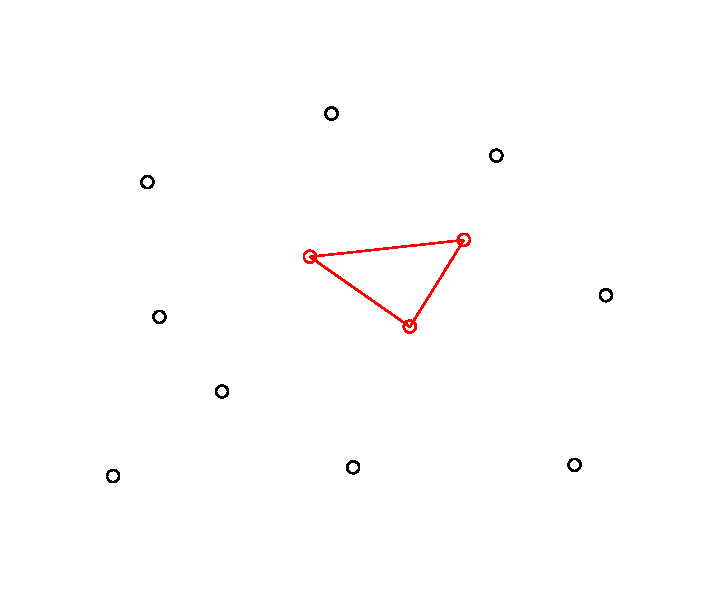
\includegraphics[width=\linewidth]{./pictures/4/incremental_hull_1.pdf}
  \label{fig:3-douglas-peucker_1}
\end{subfigure}\hfil % <-- added
\begin{subfigure}{0.5\textwidth}
  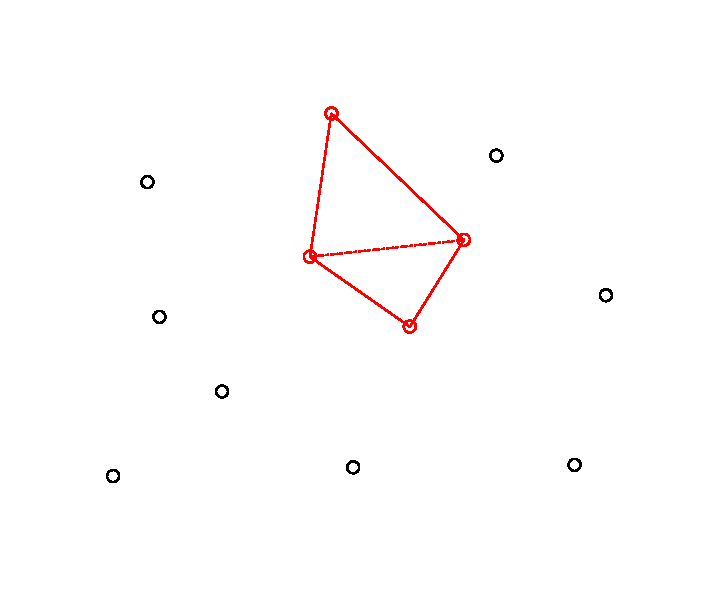
\includegraphics[width=\linewidth]{./pictures/4/incremental_hull_2.pdf}
  \label{fig:3-douglas-peucker_2}
\end{subfigure}\hfil % <-- added
\begin{subfigure}{0.5\textwidth}
  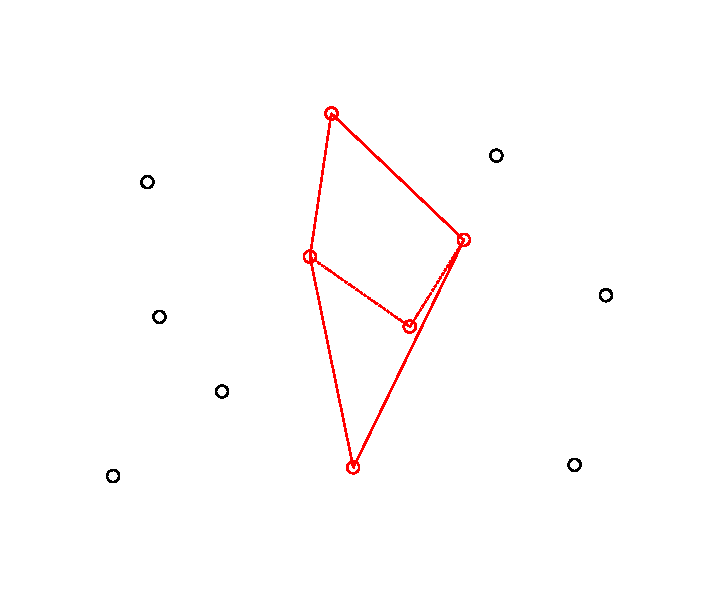
\includegraphics[width=\linewidth]{./pictures/4/incremental_hull_3.pdf}
  \label{fig:3-douglas-peucker_3}
\end{subfigure}\hfil % <-- added
\begin{subfigure}{0.5\textwidth}
  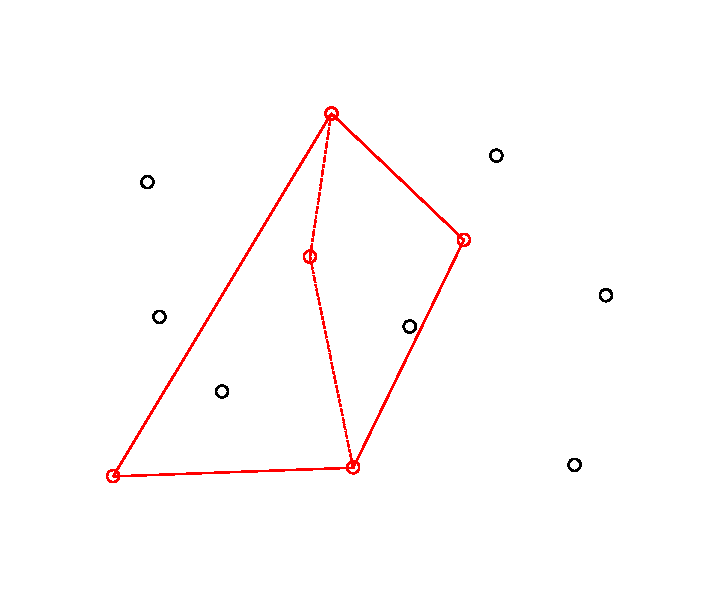
\includegraphics[width=\linewidth]{./pictures/4/incremental_hull_4.pdf}
  \label{fig:3-douglas-peucker_4}
\end{subfigure}\hfil % <-- added
\caption{Znázornění postupu inkrementálního algoritmu pro konvexní obálku}
\end{figure}